\documentclass{report}
\usepackage{hyperref}
\usepackage{listings}
\usepackage{color}
\usepackage{multirow}
\usepackage{graphicx}
\usepackage{titletoc}

\definecolor{dkgreen}{rgb}{0,0.6,0}
\definecolor{gray}{rgb}{0.5,0.5,0.5}
\definecolor{pink}{rgb}{1,0.07,0.57}


\lstset{frame=tb,
  language=Java,
  aboveskip=3mm,
  belowskip=3mm,
  showstringspaces=false,
  columns=flexible,
  basicstyle={\small\ttfamily},
  numbers=none,
  numberstyle=\tiny\color{blue},
  keywordstyle=\color{pink},
  commentstyle=\color{dkgreen},
  stringstyle=\color{blue},
  breaklines=true,
  breakatwhitespace=true
  tabsize=3
}

\lstset{language=Java}

\title{Secure Coding - Team 7- Phase 5}
\author{Magnus Jahnen, Thomas Krex, Elias Tatros}
\date{\today}


\begin{document}

\maketitle

\part{Executive Summary}

This is the final report for the Secure Coding bank web application project of Team 7. In the semester we had to develop a common bank web software with different user roles, transactions of money with different TAN methods and batch transaction via file upload.

The bank application was tested by two other teams. The aim of the tests was to find security vulnerabilities. After each test we fixed all vulnerabilities the team or we ourselves have found. As a plus we implemented new features or fixed other non security related bugs.

This final report first describes the architecture of our application. After that there is a brief overview of the security measures our system offers. The last part describes the recent fixes we have implemented.

\tableofcontents

\part{Time Tracking Table}
\chapter{Time Tracking Table}

\begin{table}[ht]
\centering
\begin{tabular}{|l|l|l|}
\hline
\multicolumn{3}{ |c| }{\textbf{Time Tracking}} \\
\hline
\textbf{Name} & \textbf{Time} & \textbf{Description} \\ \hline
\multirow{6}{*}{Magnus Jahnen} 
& 15h & Reverse engineer batch parser (team 8) \\ 
& 2h & Reverse engineer batch parser (own) \\
& 5h & Reverse engineer Java-SCS (team 8) \\ 
& 2h & Reverse engineer Java-SCS (own) \\
& 10h & Meetings \\
& 5h & Report \& Presentation \\ \hline
\multirow{6}{*}{Thomas Krex} 
& 3h & Fixes for TAN Generation
& 2h & Adjust session cookie settings \\
& 3h & Trailer \\
& 2h & Meetings \\
& 5h & Documentation \\ \hline
\multirow{6}{*}{Elias Tatros} & 2h & Static Analysis decompiled Java and PHP \\
& 4h & Finding Encryption Flaws in Java/PHP \\ 
& 5h & Analysis of application memory \\ 
& 15h & Planning, Implementation and Testing of Memory Scanner \\ 
& 6h & Working on Report (Sections on Key Weakness, Memory Scanner, Static IV)\\
& 10h & Meetings \\ \hline
\end{tabular}
\label{table:time_tracking}
\end{table}


\part{Application Architecture}
\chapter{Architecture}
In this section we take a look at the relationships and organizational structure of the internal and external components that make up the \textit{myBank} banking application. The architecture description of our application defines several separate components and sub-components, each having clearly designed responsibilities. Interaction between components is controlled through the specification of interfaces. The goal of the design was to structure the application in such a way, that it would meet all requirements of the specification, while being well documented, maintainable and easily extensible in the future.
\section{Three Layer Structure}
Figure \ref{architecture} shows the main structure of the myBank application. The \textit{Smart-Card-Simulator} (\textit{SCS}) was not included in this figure, since it is regarded as an independent external component, which does not interact with the main myBank system. From a high abstraction level view, the application is structured into a classic three layers architecture. The fundamental layer at the bottom of the hierarchy is the \textit{Data Layer}. The main responsibility of this layer is to store and retrieve data. The \textit{Data Layer} offers an interface for data storage and retrieval functions, which is used by the \textit{Logic Layer}. This layer contains the ``meat'' of the banking application (\textit {business logic}), meaning that it contains the central components of the system, which are handling all logical tasks and are not part of the supporting infrastructure. This includes components responsible for Transactions, User management, Tan generation, Email dispatch and so on. The logic layer in turn offers functionality through an interface, that is used by the \textit{Presentation Layer} to display and manipulate information on the user level. In general we made sure, that components of each layer are only allowed to use the next lower layer through a specified interface, although our application does not strictly adhere to this in all cases.
%++++++++++++++++++++++++++++++++++++++++++++++++++++++
%+    Figure 1: myBank Component Overview             +
%++++++++++++++++++++++++++++++++++++++++++++++++++++++
\begin{center}
\begin{figure}[hbtp]
        \centering
        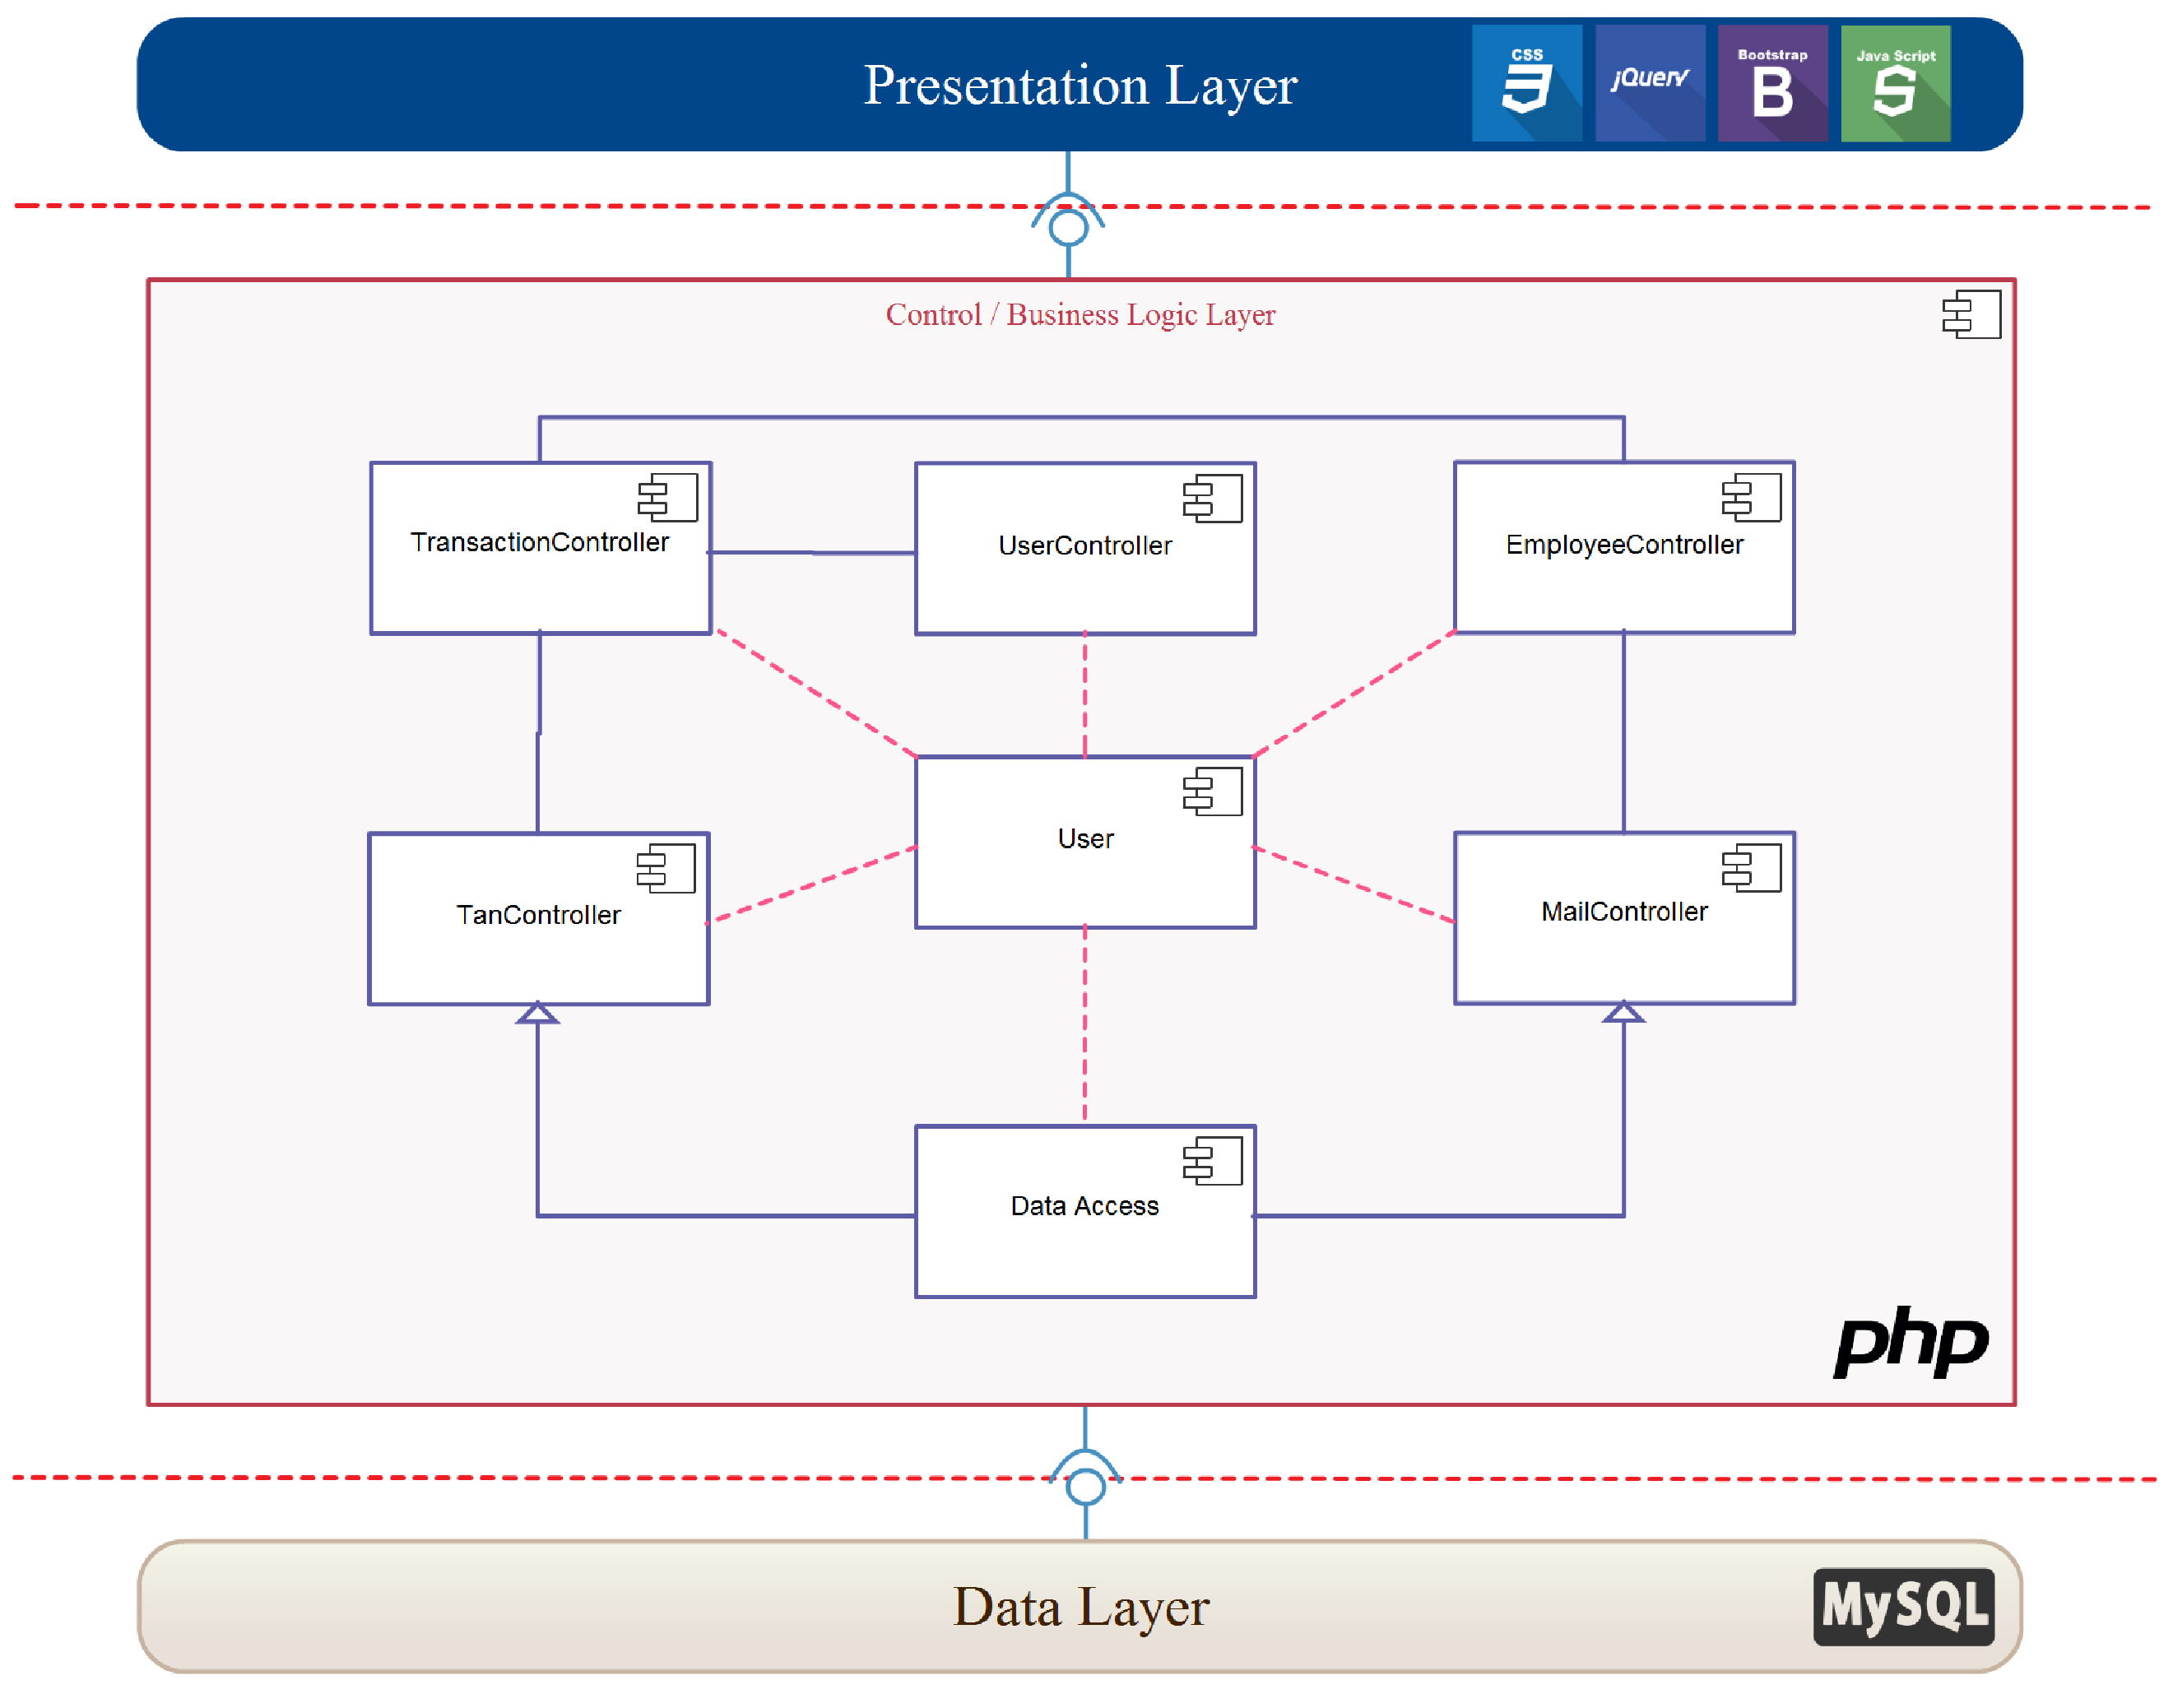
\includegraphics[width=1.0\linewidth]{architecture}
        \caption{myBank Component Overview}\label{architecture}
\end{figure}
\end{center}
\section{Logic Layer Components: Separation of Concerns}
The sub-components of the logic layer clearly encapsulate related functionality and are designed to function as independently as possible. Moreover, components and modules are clearly named according to their responsibilities. This makes a complex system easier to understand and limits the possibility for confusion, due to inappropriately named modules. The important components of the logic layer are:
\begin{itemize}

  \item Data Access
  \item User
  \item User Controller
  \item Tan Controller
  \item Transaction Controller
  \item Employee Controller
  \item Mail Controller

\end{itemize}
The flow of data is generally designed to be from bottom to top, as indicated by the arrows in figure \ref{architecture}. Dependencies between components are designed to be minimal. Most components depend on a maximum of one or two other components, which also limits their communication channels, improving maintainability and ease of use. The following list gives some insight into the functionality that is encapsulated by each of the main logic layer components. We would like to note, that we realize, the architecture is not perfect and there is still room for improving the independence of components and their modules.
\begin{description}
  \item[Data Access] \hfill \\
  Abstracts access to the data layer. Main task is insertion and retrieval of data through communication with the mysql database.
  \item[User] \hfill \\
  Abstracts a user or employee of the System. The myBank application is a user centric system, meaning that the user (customer or employee) is the central component of the system and is involved in almost all operations performed at the logic layer. Since the User class is used by nearly all sub-components, it is designed to be very concise and lightweight.
  \item[User Controller] \hfill \\
  Offers functionality to verify user and employee credentials, as well as control over the lockout mechanisms.
  \item[Tan Controller] \hfill \\
  Responsible for generation, verification, selection and maintenance of transaction numbers.
  \item[Transaction Controller] \hfill \\
  Implements functionality for credit transfers between users. Each transaction involves a large number of steps, including the validity of transaction data, verification of credentials, checking of available funds, selection of TANs and so on. These steps are abstracted into an easy to use interface by the Transaction Controller.
  \item[Employee Controller] \hfill \\
  Offers employee functionality, such as approval of users and transactions over the limit of 10000 Credits.
  \item[Mail Controller] \hfill \\
  As the name suggests, this component is tasked with sending out Emails to customers.
\end{description}
Figure \ref{hierarchy} shows a more granular view of some system modules on the function level. The figure shows a functional hierarchy for parts of the Mail Controller, User Controller and Data Access. In the body of each function dependencies are listed, some of which are external and not included in this view to abstract from the complexity.
%++++++++++++++++++++++++++++++++++++++++++++++++++++++
%+    Figure 2: myBank Functional Hierarchy           +
%++++++++++++++++++++++++++++++++++++++++++++++++++++++
\begin{center}
\begin{figure}[hbtp]
        \centering
        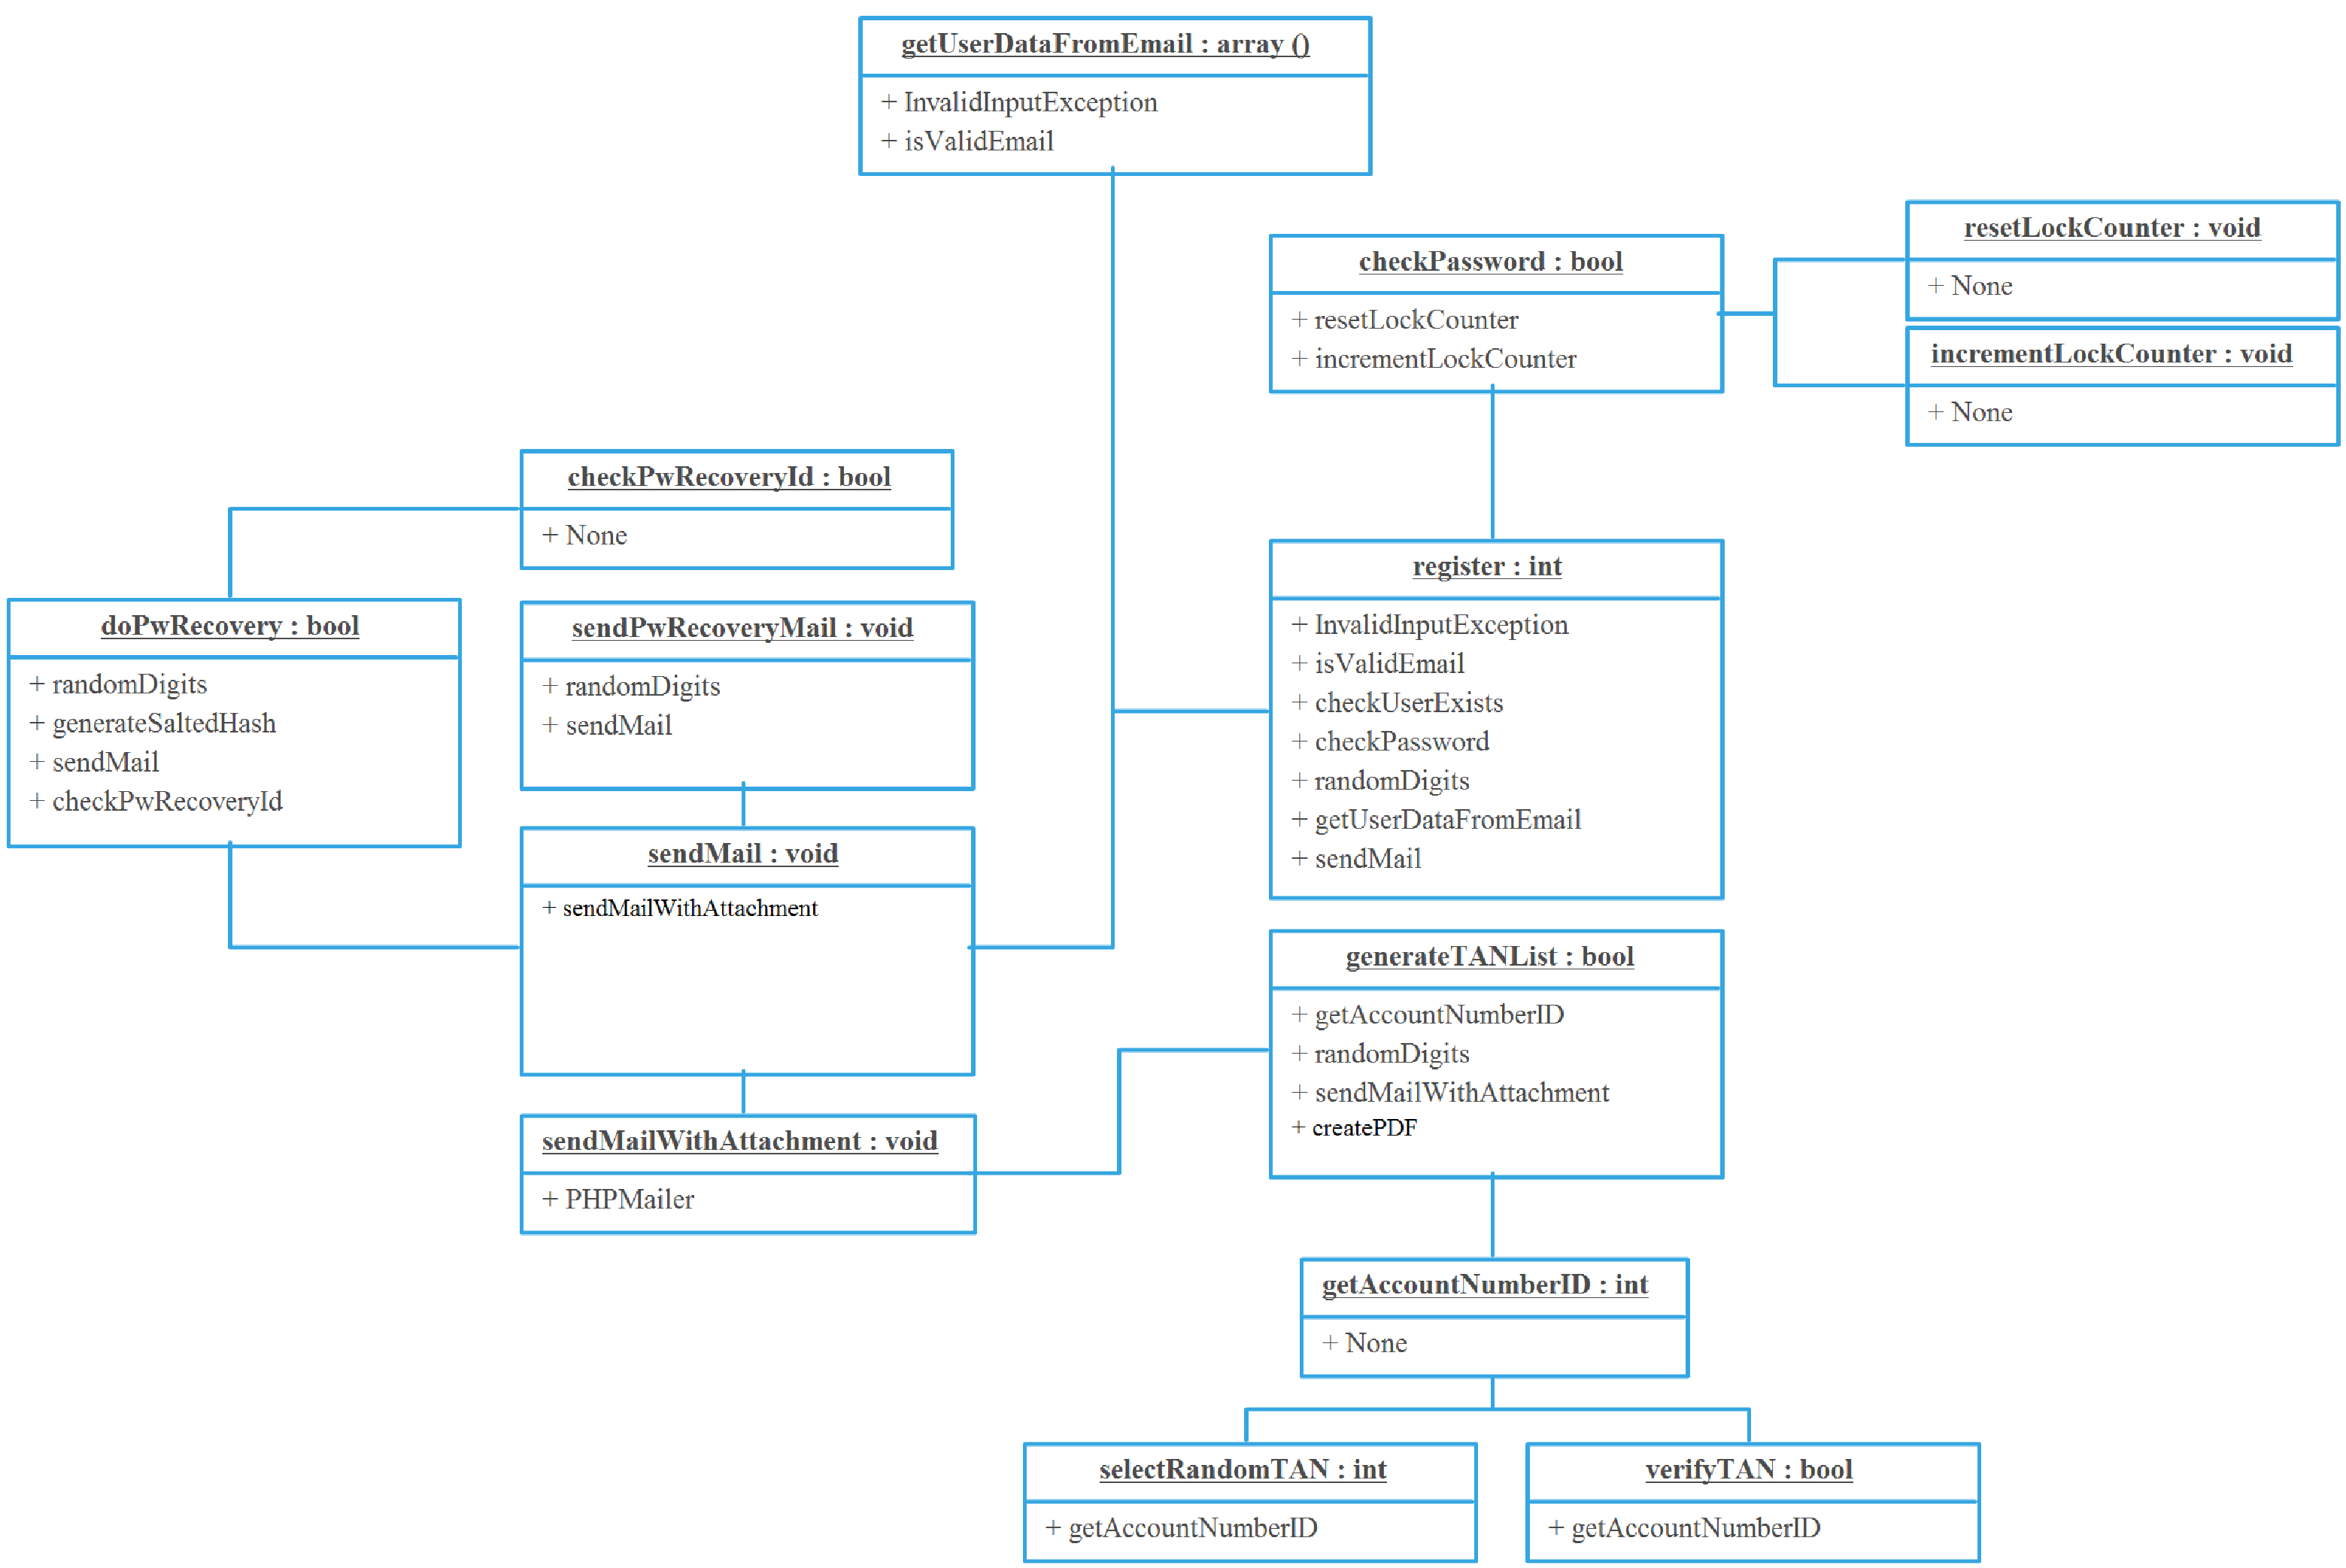
\includegraphics[width=1.0\linewidth]{hierarchy}
        \caption{myBank Function Hierarchy Excerpt}\label{hierarchy}
\end{figure}
\end{center}
\section{Technologies \& Languages}
The myBank application makes use of several different technologies on each layer. The following is a list of technologies and programming/scripting languages utilized by layer.
\begin{description}
  \item[Presentation Layer] \hfill \\
  HTML5, CSS3, JavaScript, Twitter Bootstrap (front-end framework), Yahoo! pure
  \item[Logic Layer] \hfill \\
  PHP 5.3/4, Java, C
  \item[Data Layer] \hfill \\
  MySQL
\end{description}

\part{Security Measures}
\chapter{Security Measures}

\section{PDF Password Protection}
The TAN List of our customers are password protected. That ensures that only customers themselves can access the transaction codes. To protect the pdfs we used the third party library FDPI.
\section{HTTPS}
Our webservice uses the HTTPS protocoll to encrypt all transmitted data to and from our clients.
This prevents attackers from reading sensitive data via man-in-the-middle attacks.
\section{Strong password policy}
We enforce the user to choose a strong password to minimize the possible threat outgoing from brute force attacks.
\section{Secure Session Management}
The session cookie of an user is only transmitted via HTTPS, can not be accessed via javascript and expires after 30 minutes. So attackers cannot bypass the authentication schema by stealing cookies of logged in users.
\section{Prepared Statements for SQL database}
We protected our web service against sql injections by using prepared statements for database requests.
\section{Anti-CSRF Token}
We attached an anti-CSRF token to all of our forms. This token is generated for each session and its existence \& correctness is verified upon submission of all post requests. Since external websites have no knowledge of the token value, they can not successfuly submit post requests in a CSRF attack.
\section{Protection of C Parser against Heap/Buffer Overflows}
To our knowledge there exist no possibilities for heap or stack overflows, since we tried to avoid allocating space on the heap and used secure functions for copying buffers. Also we add the compiler flag \textit{-fPIE} and \textit{-fstack-protector-all} in gcc to randomize address locations and a canary, making it harder for an attacker to cause buffer overflows.
\section{Secure TAN Generation}
To generate secure transaction codes for single or batch transfers, we use the hash algorithm sha256 in combination with a current timestamp as seeed. Time syncrhonization is done via a NTP server. The timestamp is concatenated with information of one transfer, including the destination account, the amount that will be transferred and the PIN of the user. A hash of this information is than trimmed to 15 digits. 
Since the timestamp is part of the TAN, one transaction code is only valid for at maximum 2 minutes, because the webservice only generates two tans for verifcation. One with the current timestamp and one with a timestamp one minute in future. Therefore transaction codes which an attacker stole, are useless in less than 2 minutes. That minimizes the risk of unauthorized transactions.
\section{Secure Password Recovery}
The Password Recovery for users is done in 3 steps. The user requests a new password at the website. Then he receives an email with a personalized URL. By clicking on it , the user gets to the page where he have to select one of the predefined security question and the corresponding answer that he specified at the registration. This procedure ensures that only the owner of the account can change the password. 
\section{Obfuscation of SCS} 
The Byte Code of the Java application SCS.jar was obfuscated with ProGuard in order to complicate the reverse engineering.
In Listing \ref{listing:proguard}, the corresponding ProGuard config is shown.

\begin{lstlisting}[caption=Configuration File of ProGuard, label=listing:proguard]
-injars /Volumes/MacintoshHD/Users/mep/Downloads/scs/scs.jar
-outjars /Volumes/MacintoshHD/Users/mep/Downloads/scs/scs_out.jar
	
-libraryjars /Library/Java/JavaVirtualMachines/jdk1.7.0_71.jdk/Contents/Home/jre/lib/rt.jar
	
-libraryjars /Library/Java/JavaVirtualMachines/jdk1.7.0_71.jdk/Contents/Home/jre/lib/jfxrt.jar
	
-dontshrink
-dontwarn com.javafx.**
-dontwarn org.apache.**
	
-keepattributes '*Annotation*'
	
-adaptresourcefilecontents **.fxml
-keepclassmembernames class * {
	@javafx.fxml.FXML *;
}
	
-keepclasseswithmembers public class com.javafx.main.Main, scs.Main {
	public *; public static *;
}
	
	
# Keep - Applications. Keep all application classes, along with their 'main'
# methods.
-keepclasseswithmembers public class * {
	public static void main(java.lang.String[]);
}
\end{lstlisting}

\section{Secure Handling of uploaded files}
Uploaded Files for batch transaction are handled in a secure manner to avoid damage done by uploaded malicious code. This includes the usage of the default PHP temporary folder. All files are stored in /tmp and get a randomly chosen name. This has two effects. First of all files are not stored at the webroot and can not be access via an unsecure webserver. Secondly, renaming files before passing them to the c parser, prevents malicous code in the filename to be executed.
\newline
Another precoution we took, is to delete this files right after parsing them, so that malicous code can't be executed on our server later on. 

\section{Lock Out Mechanism}

To avoid Brute Force attacks, we implemented an lock out mechanism at login and when entering TANs.

Hence the a user will be blocked after a certain count of invalid inputs. After that no further login is possible for the user and he must be approved again by an employee.





\part{Fixes}
\chapter{Fix of HTTP Strict Transport Security}
\section{Affected Files}

/etc/apache2/httpd.conf: line 15

\section{Description}

We added an HTTP Scrict Transport Security Header to teh config of our web server. Therefore the server notifies the client's browser that all traffic has to be exchanged via HTTPS.
To do so the added the following line to the Virtual Host Config:

Header add Strict-Transport-Security "max-age=15768000"


\chapter{Fix for Bypassing Session Management Schema and Cookies attributes}
\section{Affected Files}

\begin{itemize}
\item /etc/apache2/httpd.conf lines: 2++
\end{itemize}

\section{description}
In order to protect the session cookie and its attributes against attackers the added the following settings to httpd.conf:

\begin{lstlisting}
	    php_value session.cookie_httponly true
	    php_value session.cookie_secure true
	    php_value session.cookie_lifetime 1800
\end{lstlisting}

The httponly flag was already set in phase 3 and prevents that the cookie can be acessed by javascript.
The http_secure flag ensures that cookies are only sent via HTTPS. \newline
Futhermore the attribute cookie_lifetime defines the expire data for a cookie. A short lifetime decreases the chances for an attacker to sucessfully use a foreign session cookie to authenticate with the web service.



\chapter{Fix Process Timing}
\section{Affected Files}
\begin{itemize}
	\item webroot/pw\_recovery.php: 137++
\end{itemize}
\section{Description}

Our App was leaking information by its process timing. To be more precise, the vulnerability was placed in the password recovery service. The User can enter his/her email address and will retrieve an email with instruction on how to change his password. The problem was the time, the system took to send that email. If entering an email which isn't registered in the system, the process takes round about 30 ms instead of 3 seconds. This means that an attacker can guess regitered email addresses my observing the process time. To fix this problem there is more than one solution. You could start an asynchronous task that is sending the mail while the web service is responding to the client. For that you have to use external libraries that would increase the complexity of the system. Another way would be to send a curl request to an internal web service. This basically would work but it requires a static host name to do so. So we decided to choose a third solution. We inserted a sleep command that will wait a randomly picked interval between two and four seconds if the email address is not known to the system. This prevents an attacker of easily guessing registered email adresses.

\begin{lstlisting}[caption=Random Timeout in pw\_recovery.php,label=listing:timeout]
	if($user->email) {
	// if we found the mail it is a valid user
	$user->sendPwRecoveryMail();
	}
	else {
	// timeout , so it's not that easy to guess existing accounts via the processing time.
	$timeout = rand(2,4);
	sleep($timeout);
	}
\end{lstlisting}
\chapter{Fix of TAN Generation}
\section{Affected Files}
\begin{itemize}
	\item c\_user.php : line 324++
	\item helper.php : line 216
\end{itemize}

\section{Description}

Our app offers the possibility to use a SmartCardSimulator to generate transaction codes for single or batch transactions. This code can then be entered at our website or in the batch transaction batch file.
To verify the TAN, the webservice is using the same computations as the SCS. This includes the hashing of a string containing the current time as seed, the destination account, the amount and the pin of the user. This String was hashed with md5. This was a vulnerability because md5 is not secure in terms of collision attacks. So we changed the hashing algorithm to sha256 which generates a 256 bit long hash instead of 128 bit. To receive the same results as the java code and the c code for parsing batch files, we had to modify the hashing, shown in Listing \ref{listing:sha256}. The hash function returns a string with a 128 bit  hexadecimal number. 16 of this 32 characters are pairwaised concatenated and transformed into decimal numbers. Because this process ingores possible signed numbers, each decimal number greater than 127 and to be substracted by 256. Of these rsulting numbers the absolute values of the first 16 numbers is concatenated and trimmed to 15 characters.   \newline
\newline

\begin{lstlisting}[caption = Generation of a TAN using sha256, label=listing:sha256]
	function generateTanWithSeed($seed,$pin,$destination,$amount){
	
	$plaintext = $seed.$pin.$destination.$amount.$seed;
	//$hash = $this->generateMD5Hash($plaintext);
	$hash = hash('sha256',$plaintext);
	$hash_array = array();
	for ($i=0;$i<16;$i += 2) {
	$tmp = substr($hash, $i,1).substr($hash, $i+1,1);
	array_push($hash_array, hexdec($tmp));
	}
	$hash_string = "";
	for ($j=0;$j<16;$j++) {
	$tmp = $hash_array[$j];
	if ($tmp > 127) {
	$tmp -= 256;
	}
	$hash_string .= strval(abs($tmp));
	}
	return substr($hash_string,0,15);
	}
\end{lstlisting}
The next problem was the  unavailbility of the time server which was used to synchronize the SCS and the webservice. Also it ensures that transaction codes for an transaction with the same amount and destinations differs over the time. This results in a stronger protecion against brutforcing the transaction codes. 
To fix this problem we simply changed the time server from that the time is requested, shown in Listing \ref{listing:time.}

\begin{lstlisting}[caption= New TimeServer IP, label=listing:time]
	function getUTCTime(){
	$timeserver = "129.6.15.28";
\end{lstlisting}
\section{Fix for Upload of Unexpected File Types}
Our app allows the user to upload any kind file for the batch transaction. But in our point of view that is nota vulnerability. Uploaded Files are not stored in the webroot of the server and are renamed before they are stored. Furthermore uplaod files are directly deleted after being parsed by the c program.
If an attacker woud have the possibility to to execute his code, the extension of the file would not make any difference.
To sum it up, allowing uploading any file extension increases the comfort of the user and has no influence on the security of our web service.
\chapter{Lock out Mechanism}

To avoid brute forcing attacks when logging in and transferring money (TANs) we implemented a mechanism which blocks the user after 5 attempts with invalid input. Thus we created a new database field in the \textit{users} table (lock\_counter, int). 

\section{Affected Files}
\begin{itemize}
	\item c\_user.php : line 898 new methods
	\item c\_user.php : lines 455, 469, 877  method call resetLockCounter()
	\item c\_user.php : lines 459, 472, 883  method call incrementLockCounter()
\end{itemize}

\section{Additions}

\begin{lstlisting}[caption = New methods]
function incrementLockCounter() {
	$connection = new PDO( DB_NAME, DB_USER, DB_PASS );
	$sql = "SELECT lock_counter FROM users WHERE email = :email LIMIT 1";
	$stmt = $connection->prepare( $sql );
	$stmt->bindValue( "email", $this->email, PDO::PARAM_STR );
	$stmt->execute();
	$result = $stmt->fetch();
	if ($result['lock_counter'] < 5) {
		$sql = "update users set lock_counter = lock_counter + 1 where email = :email";
		$stmt = $connection->prepare( $sql );
		$stmt->bindValue( "email", $this->email, PDO::PARAM_STR );
		$stmt->execute();
		return false;
	} else {
		$sql = "update users set is_active = 0, lock_counter = 0 where email = :email";
		$stmt = $connection->prepare( $sql );
		$stmt->bindValue( "email", $this->email, PDO::PARAM_STR );
		$stmt->execute();
		return true;
	}
	
	$connection = null;
}
function resetLockCounter() {
	$connection = new PDO( DB_NAME, DB_USER, DB_PASS );
	$sql = "update users set lock_counter = 0 where email = :email";
	$stmt = $connection->prepare( $sql );
	$stmt->bindValue( "email", $this->email, PDO::PARAM_STR );
	$stmt->execute();
	$connection = null;
}
\end{lstlisting}
\chapter{Security Question for Password Recovery}

In Phase 3 we developed a password recovery functionality, which sends the user a generated new password via email. Because the user had no opportunity to change the password it would be easy for an attacker to log into any account if he somehow could get the user's emails.

Therefore we included a security question in the registration process, the user must answer correctly when recovering his password.

We added two database fields into the \textit{users} table. The number of the security question the user chose, can be between 0 and 4 and the answer of the question are saved in them.

\section{Diff}

\begin{lstlisting}[caption = c\_user.php]
line 26
+	public $securityQuestionNumber = null;
+	public $securityQuestionAnswer = null;
line 550
+		
+		if( isset( $data['sec_q_number'] ) ) {
+			$this->securityQuestionNumber = stripslashes( strip_tags( $data['sec_q_number'] ) );
+		} else {
+			throw new InvalidInputException("Security Question not specified.");
+		}
+		
+		if( isset( $data['sec_q_answer'] ) ) {
+			$this->securityQuestionAnswer = stripslashes( strip_tags( $data['sec_q_answer'] ) );
+		} else {
+			throw new InvalidInputException("Security Question Answer not specified.");
+		}

line 571
-			$sql = "INSERT INTO users (email,name,passwd,is_employee,is_active,pin,use_scs) VALUES (:email,:name,:password,:isEmployee,:isActive,:pin,:use_scs)";
+			$sql = "INSERT INTO users (email,name,passwd,is_employee,is_active,pin,use_scs,security_question_number,security_question_answer) VALUES (:email,:name,:password,:isEmployee,:isActive,:pin,:use_scs,:security_question_number,:security_question_answer)";

line 592
+			$stmt->bindValue( "use_scs", $this->useScs, PDO::PARAM_STR );
+			$stmt->bindValue( "security_question_number", $this->securityQuestionNumber, PDO::PARAM_STR );
+			$stmt->bindValue( "security_question_answer", $this->securityQuestionAnswer, PDO::PARAM_STR );

line 745
-			$sql = "SELECT id, name, use_scs, email, passwd, pin, BIN(`is_employee` + 0) AS `is_employee`, BIN(`is_active` + 0) AS `is_active`, pw_recover_id FROM users WHERE email = :email LIMIT 1";
+			$sql = "SELECT id, name, use_scs, email, passwd, pin, BIN(`is_employee` + 0) AS `is_employee`, BIN(`is_active` + 0) AS `is_active`, pw_recover_id, security_question_number, security_question_answer FROM users WHERE email = :email LIMIT 1";
 
 line 764
 +			$this->securityQuestionNumber = $result['security_question_number'];
 +			$this->securityQuestionAnswer = $result['security_question_answer'];
 
 line 790
 -			$sql = "SELECT id, name, email, passwd, use_scs, pin, BIN(`is_employee` + 0) AS `is_employee`, BIN(`is_active` + 0) AS `is_active`, pw_recover_id FROM users WHERE id = :id LIMIT 1";
 +			$sql = "SELECT id, name, email, passwd, use_scs, pin, BIN(`is_employee` + 0) AS `is_employee`, BIN(`is_active` + 0) AS `is_active`, pw_recover_id, security_question_number, security_question_answer FROM users WHERE id = :id LIMIT 1";
  	
line 808
+			$this->securityQuestionNumber = $result['security_question_number'];
+			$this->securityQuestionAnswer = $result['security_question_answer'];
 	
line 1195
-	public function doPwRecovery($id) {
+	public function checkPwRecoveryId($id) {
 		
 		if(!is_numeric($id))
 			return false;
-		if(strcmp($this->pwRecoverId, $id) == 0) {
-			$newPassword = randomDigits(8);
 			
-			try {
-				$connection = new PDO( DB_NAME, DB_USER, DB_PASS );
-				$sql = "UPDATE users set passwd = :password, pw_recover_id='NULL' WHERE id = :id";
-		
-				$stmt = $connection->prepare( $sql );
-				$stmt->bindValue( "password", generateSaltedHash($newPassword), PDO::PARAM_STR );
-				$stmt->bindValue( "id", $this->id, PDO::PARAM_STR );
-				$stmt->execute();
-		
-				$connection = null;
+		return strcmp($this->pwRecoverId, $id) == 0;
+	}
+	
+	public function doPwRecovery($id, $postArray) {
+		if(!$this->checkPwRecoveryId($id)) 
+			return false;
-				// Send the mail
+		if(strcmp($this->securityQuestionAnswer, $postArray['sec_q_answer']) != 0) {
+			return false;
+		}
+		
+		try {
+			$connection = new PDO( DB_NAME, DB_USER, DB_PASS );
+			$connection->setAttribute( PDO::ATTR_ERRMODE, PDO::ERRMODE_EXCEPTION );
-				$message= "your new Password is: $newPassword";
-				
-				$this->sendMail($this->email, $message, "Your new Password");
-				
-				return true;
+			$sql = "update users set passwd = :password, pw_recover_id = NULL where id = :id";
} catch ( PDOException $e ) {
-				echo "<br />Connect Error: ". $e->getMessage();
-				return false;
-			}
+			$stmt = $connection->prepare( $sql );
+			$stmt->bindValue( "password", generateSaltedHash($postArray['password']), PDO::PARAM_STR );
+			$stmt->bindValue( "id", $this->id, PDO::PARAM_STR );
+			$stmt->execute();

-		} else {
+			return true;
+		} catch ( PDOException $e ) {
+			echo "<br />Connect Error: ". $e->getMessage();
 			return false;
 		}
-		
 	}
\end{lstlisting}

\begin{lstlisting}[caption = conf.php]
line 9
$SECURITY_QUESTIONS = array("What is the first name of the person you first kissed?",
+				"What is the last name of the teacher who gave you your first failing grade?",
+				"What is the name of the place your wedding reception was held?",
+				"In what city or town did you meet your spouse/partner?",
+				"What was the make and model of your first car?" );
 
\end{lstlisting}


\begin{lstlisting}[caption = register.php]
line 74
+		        <div class="pure-control-group">
+				<label for="sec_q_number">Security Question (Needed for Password recovery)</label>
+		        <select id="sec_q_number" name="sec_q_number" size="1">
+				<?php 
+					$counter = 0;
+					foreach($SECURITY_QUESTIONS as $question) {
+						echo "<option value=\"$counter\">$question</option>";
+						$counter = $counter +1;
+					}
+				?>
+			    </select>
+		        </div> 
+		        
+		        
+		        <div class="pure-control-group">
+		            <label for="sec_q_answer">Answer</label>
+		            <input name="sec_q_answer" id="sec_q_answer" type="text" placeholder="Answer" onkeyup="check_answer()" required>
+		            <b id=answer_info></b>
+		        </div>
+		        

line 175
+	function check_answer() {
+		var an_field = document.getElementById("sec_q_answer")
+		var an_info = document.getElementById("answer_info")
+		
+		if (an_field.value.length >= 4) {
+			submit_button.disabled = false;
+			an_info.textContent = ""
+		} else {
+			submit_button.disabled = true;
+			an_info.textContent = "Answer must be at least 4 characters"
+		}
+	}
+	
\end{lstlisting}

\begin{lstlisting}[caption = pw\_recovery.php]
line 22
+	
 	$user = new User();
 	$user->getUserDataFromEmail($_GET['email']);
+	
+	
+	if( isset($_POST['password'])) {
+		if($user->doPwRecovery($_GET['id'], $_POST))
+			echo "Success, your password was set to the newly entered one!";
+		else
+			echo "Something went wrong, please try again later!";
+			
+		die();
+	}
+	
 	$success = false;
 	if($user->email) {
 		// if we found the mail it is a valid user
-		$success = $user->doPwRecovery($_GET['id']);
+		$success = $user->checkPwRecoveryId($_GET['id']);
 	}?>
 	
line 65
<p>
 			<?php 
 			if($success) {
-				echo "Your new password has been sent to you via email!";
+			?>
+			<form method="post" action="" class="pure-form pure-form-aligned">
+		    <fieldset>
+				<div class="pure-control-group">
+				<label for="sec_q_number">Security Question:</label>
+		        <label name="sec_q_number" id="sec_q_number"><?php echo $SECURITY_QUESTIONS[$user->securityQuestionNumber] ?></label>
+		        </div> 
+		        
+		        
+		        <div class="pure-control-group">
+		            <label for="sec_q_answer">Answer</label>
+		            <input name="sec_q_answer" id="sec_q_answer" type="text" placeholder="Answer" required>
+		        </div>
+		        
+		        <div class="pure-control-group">
+		            <label for="password">New Password</label>
+		            <input name="password" id="password" type="password" placeholder="***********" onkeyup="check_pw()" required>
+		            <b id=password_info></b>
+		        </div>
+		        
+		        <div class="pure-control-group">
+		            <label for="confirm_password">Confirm Password</label>
+		            <input name="confirm_password" id="confirm_password" type="password" placeholder="***********" onkeyup="check_pw()" required>
+		            <b id=confirm_password_info></b>
+		        </div>
+		        
+		        <div class="pure-controls">
+		            <button id="SendButton" type="submit" name="recoverPassword" class="pure-button pure-button-primary" onclick="setTimeout(disableFunction, 1);">Submit</button>
+		        </div>
+		        
+		    </fieldset>
+			</form>
+			<?php 

line 153
-	<script>
-		function disableFunction() {
-		    document.getElementById("SignInButton").disabled = 'true';
-		}
-	</script>

line 213
+
+	<script>
+		function disableFunction() {
+		    document.getElementById("SignInButton").disabled = 'true';
+		}
+		
+		var pw_info = document.getElementById("password_info")
+	var confirm_pw_info = document.getElementById("confirm_password_info")
+	
+	var pw_field = document.getElementById("password")
+	var confirm_pw_field = document.getElementById("confirm_password")
+	
+	var submit_button = document.getElementById("SendButton")
+	submit_button.disabled = true
+	
+	function check_pw() {
+		// lets check if the pw is strong enough
+		var pw = pw_field.value
+		var lowercase = pw.search("[A-Z]")
+		var uppercase = pw.search("[a-z]")
+		var number = pw.search("[0-9]")
+		
+		if(pw.length < 8 || lowercase == -1 || uppercase == -1 || number == -1) {
+			pw_info.textContent = "Password must have at least eight characters, one upper case, one lower case letter and one number"
+			submit_button.disabled = true
+		} else {
+			pw_info.textContent = ""
+		}
+	
+		if(confirm_pw_field.value != pw_field.value) {
+			confirm_pw_info.textContent = "The two passwords do not match!"
+			submit_button.disabled = true
+		} else {
+			confirm_pw_info.textContent = ""
+			submit_button.disabled = false
+		}
+	}
+
+	</script>
\end{lstlisting}

\end{document}